\let\negmedspace\undefined
\let\negthickspace\undefined
\documentclass[journal,12pt,onecolumn]{IEEEtran}
\usepackage{cite}
\usepackage{amsmath,amssymb,amsfonts,amsthm}
\usepackage{algorithmic}
\usepackage{graphicx}
\graphicspath{{./figs/}}
\usepackage{textcomp}
\usepackage{xcolor}
\usepackage{txfonts}
\usepackage{listings}
\usepackage{enumitem}
\usepackage{mathtools}
\usepackage{gensymb}
\usepackage{comment}
\usepackage{caption}
\usepackage[breaklinks=true]{hyperref}
\usepackage{tkz-euclide} 
\usepackage{listings}
\usepackage{gvv}                                        
%\def\inputGnumericTable{}                                 
\usepackage[latin1]{inputenc}     
\usepackage{xparse}
\usepackage{color}                                            
\usepackage{array}                                            
\usepackage{longtable}                                       
\usepackage{calc}                                             
\usepackage{multirow}
\usepackage{multicol}
\usepackage{hhline}                                           
\usepackage{ifthen}                                           
\usepackage{lscape}
\usepackage{tabularx}
\usepackage{array}
\usepackage{float}
\newtheorem{theorem}{Theorem}[section]
\newtheorem{problem}{Problem}
\newtheorem{proposition}{Proposition}[section]
\newtheorem{lemma}{Lemma}[section]
\newtheorem{corollary}[theorem]{Corollary}
\newtheorem{example}{Example}[section]
\newtheorem{definition}[problem]{Definition}
\newcommand{\BEQA}{\begin{eqnarray}}
	\newcommand{\EEQA}{\end{eqnarray}}
\newcommand{\define}{\stackrel{\triangle}{=}}
\theoremstyle{remark}
\newtheorem{rem}{Remark}

\newcommand{\ihat}{\mathbf {\hat \imath}}
\newcommand{\jhat}{\mathbf {\hat \jmath}}
\newcommand{\vect}[1]{\mathbf #1}



\title{CH: CHEMICAL ENGINEERING}
\author{EE25BTECH11042 - Nipun Dasari}
\date{   }


\begin{document}
	
	\bibliographystyle{IEEEtran}
	\vspace{3cm}
	
	\maketitle
	
	\begin{enumerate}
		\item The direction of largest increase of the function xy\textsuperscript{3} - x\textsuperscript{2} the point \brak{1,1} is - 
		\begin{enumerate}
			\begin{multicols}{4}
				
				
				\item  	
				
				$ 3\ihat + 4\jhat$
				
				\item 
				
				$3\ihat + 4\jhat$
				
				\item 
				
				$3\ihat + 4\jhat$
				
				\item  
				
				$3\ihat + 4\jhat$
			\end{multicols}
		\end{enumerate}
		
		
		\hfill \brak{\text{GATE CH 2009}}
		
		
		
		\item The modulus of the complex number is \brak{1 + i}/$\sqrt{2}$ 
		\begin{enumerate}
			\begin{multicols}{4}
				\item 1/2
				\item 1/$\sqrt{2}$
				\item 1
				\item $\sqrt{2}$
			\end{multicols}
		\end{enumerate} 
		
		\hfill \brak{\text{GATE CH 2009}}
		
		
		\item The system of linear equations $\vec{Ax = 0}$, where $\vec{A}$ is an nxn matrix, has a non-trivial solution ONLY if-
		
		\begin{enumerate}
			\begin{multicols}{2}
				\item rank of $\vec{A}$$>$n
				\item rank of $\vec{A}$$=$n
				\item rank of $\vec{A}$$<$n
				\item $\vec{A}$ is an identity matrix
			\end{multicols}
		\end{enumerate}
		
		\hfill \brak{\text{GATE CH 2009}}
		
		\item A dehumidifier \brak{\text{shown below}} is used to completely remove water vapour from air
		\begin{figure}[H]
			\centering
			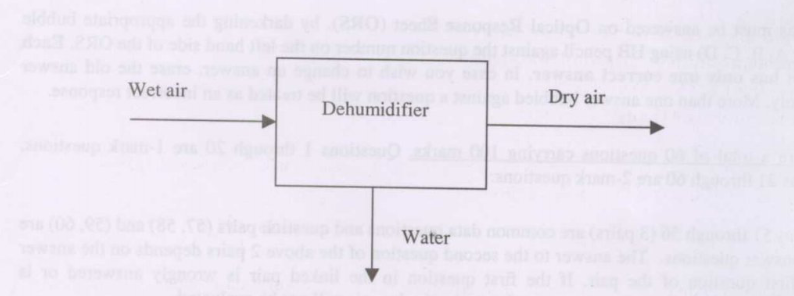
\includegraphics[width = 0.7\columnwidth]{q4.png}
			\caption{}
			\label{fig:q4}
		\end{figure}
		Which \textbf{ONE} of the following statements is \textbf{TRUE} 
		\begin{enumerate}
			
			\item  Water is the ONLY tie component
			\item Air is the ONLY tie component
			\item BOTH water and air are tie components
			\item There are NO tie components
			
		\end{enumerate} 
		
		\hfill \brak{\text{GATE CH 2009}}
		
		\item Dehydrogenation of ethane, $ H_6$ \brak{g} $/rightarrow$ $ H_4$ \brak{g} + $H_2$ \brak{g}, is carried out in a continuous stirred tank reactor \brak{\text{CSTR}} The feed is pure ethane. If the reactor exit stream contains unconverted ethane along with the products, then the number of degrees of freedom for the CSTR is 
		\begin{enumerate}
			\begin{multicols}{4}
				\item 1
				\item 2
				\item 3
				\item 4
			\end{multicols}
		\end{enumerate} 
		
		\hfill \brak{\text{GATE CH 2009}}
		
		\item An ideal gas at temperature $T_{1}$ and pressure $P_{1}$ is compressed isothermally to pressure $P_{2}$ \brak{> P_{1}} in a closed system. Which ONE of the following is TRUE for internal energy \brak{U} and Gibbs free energy \brak{G} of the gas at the two states? 
		\begin{enumerate}      
			\begin{multicols}{2}
				\item   $U_1= U_2$,  $G_1$> $G_2$   
				\item   $U_1$=$ U_2$,  $G_1$< $G_2$
				\item   $U_1$>$ U_2$,  $G_1= G_2  $  
				\item   $U_1$<$ U_2$,$  G_1= G_2$
			\end{multicols}
		\end{enumerate} 
		
		\hfill \brak{\text{GATE CH 2009}}
		
		
		
		\item Under fully turbulent flow conditions, the frictional pressure drop across a packed bed varies with the superficial velocity \brak{V} of the fluid as - 
		\begin{enumerate}
			\begin{multicols}{4}
				\item $V^{-1}$
				\item V
				\item $V^{3/2}$
				\item $V^2$
			\end{multicols}
		\end{enumerate} 
		
		\hfill \brak{\text{GATE CH 2009}}
		
		\item For a mixing tank operating in the laminar regime, the power number varies with the Reynolds number \brak{Re} as
		\begin{enumerate}
			\begin{multicols}{4}
				\item $Re^\frac{-1}{2}$
				\item $Re^\frac{1}{2}$
				\item Re
				\item $Re^-1$
			\end{multicols}
		\end{enumerate} 
		
		\hfill \brak{\text{GATE CH 2009}}
		
		\item During the transient convective cooling of a solid object, Biot number $\rightarrow$ O indicates 
		\begin{enumerate}
			\item uniform temperature throughout the object
			\item negligible convection at surface of the object
			\item significant thermal resistance within the object
			\item significant temperature gradient within the object
		\end{enumerate} 
		
		\hfill \brak{\text{GATE CH 2009}}
		
		\item The Prandtl number of a fluid is the ratio of 
		\begin{enumerate}
			\item thermal diffusivity to momentum diffusivity
			\item momentum diffusivity to thermal diffusivity
			\item conductive resistance to convective resistance
			\item thermal diffusivity to kinematic viscosity
		\end{enumerate} 
		
		\hfill \brak{\text{GATE CH 2009}}
		
		\item According to the penetration theory of mass transfer, the mass transfer coefficient \brak{k} varies with diffusion coefficient \brak{D} of the diffusing species as 
		\begin{enumerate}
			\begin{multicols}{4}
				\item  D
				\item  $D^\frac{-1}{2}$
				\item  $D^\frac{1}{2}$
				\item $D^\frac{3}{2}$
			\end{multicols}
		\end{enumerate} 
		
		\hfill \brak{\text{GATE CH 2009}}
		
		\item The ratio of the liquid to gas flow rate in a counter-current gas absorption column is increased, at otherwise identical conditions. Which ONE of the following statements is TRUE ? 
		\begin{enumerate}
			\item  The operating line shifts towards the equilibrium curve
			\item  The operating line shifts away from the equilibrium curve
			\item  The concentration of the absorbed species increases in the exit liquid stream
			\item The operating line does not shift
		\end{enumerate} 
		
		\hfill \brak{\text{GATE CH 2009}}
		
		\item For a homogeneous reaction system, where
		
		$C_{j}$ is the concentration of j at time t
		$N_{j}$ is the number of moles of j at time t
		V is the reaction volume at time t
		1 is the reaction time
		The rate of reaction for species j is defined as 
		\begin{enumerate} 
			\begin{multicols}{4}
				\item $\frac{dC_{j}}{dt}$
				\item  - $\frac{dC_{j}}{dt}$
				\item $\frac{1}{V}$$\frac{dN_{j}}{dt}$
				\item -$\frac{1}{V}$$\frac{dN_{j}}{dt}$
			\end{multicols}
		\end{enumerate}
		
		\hfill \brak{\text{GATE CH 2009}}
		
		\item The half-life of a first order liquid phase reaction is 30 seconds. Then the rate constant, in min\textsuperscript{-1}, is 
		\begin{enumerate}
			\item 0.0231
			\item 0.602
			\item 1.386
			\item2.0
		\end{enumerate} 
		
		\hfill \brak{\text{GATE CH 2009}}
		
		\item For a solid catalyzed reaction, the Thiele modulus is proportional to 
		\begin{enumerate}
			\begin{multicols}{2}
				\item $\sqrt{\frac{\text{intrinsic reaction rate}}{{\text {diffusion rate}}}}$
				\item $\sqrt{\frac{\text{diffusion rate}}{\text{intrinsic reaction rate}}}$
				\item ${\frac{\text{intrinsic: reaction rate}}{\text{diffusion: rate}}}$
				\item ${\frac{\text{diffusion rate}}{\text{intrinsic: reaction rate}}}$
			\end{multicols}
		\end{enumerate} 
		
		\hfill \brak{\text{GATE CH 2009}}
		
		\item  Which ONE of the following sensors is used for the measurement of temperature in a combustion process \brak{T>1800\degree C} ?
		\begin{enumerate}
			\item  Type J thermocouple
			\item  Thermistor
			\item  Resistance temperature detector
			\item Pyrometer
		\end{enumerate} 
		
		\hfill \brak{\text{GATE CH 2009}}
		
		\item The roots of the characteristic equation of an underdamped second order system are 
		\begin{enumerate}
			\item  real, negative and equal
			\item  real, negative and unequal
			\item  real, positive and unequal
			\item complex conjugates
		\end{enumerate} 
		
		\hfill \brak{\text{GATE CH 2009}}
		
		\item The total fixed cost of a chemical plant is Rs. 10.0 lakhs; the internal rate of return is 15 per cent and annual operating cost is rs. 2.0 lakhs. The annualised cost of plant is 
		\begin{enumerate}
			\begin{multicols}{4}
				\item  1.8
				\item  2.6
				\item  3.5
				\item  4.3
			\end{multicols}
		\end{enumerate} 
		
		\hfill \brak{\text{GATE CH 2009}}
		
		\item In petroleum refining operations, the process used for converting paraffins and naphthenes to aromatics is 
		\begin{enumerate}
			\begin{multicols}{2}
				\item  catalytic reforming
				\item  catalytic cracking
				\item  hydrocracking
				\item  alkylation
			\end{multicols}
		\end{enumerate} 
		
		\hfill \brak{\text{GATE CH 2009}}
		
		\item The active component of catalysts used in steam reforming of methane to produce synthesis gas is 
		\begin{enumerate}
			\begin{multicols}{4}
				\item  Nickel
				\item  Iron
				\item  Platinum
				\item  Palladium
			\end{multicols}
		\end{enumerate} 
		
		\hfill \brak{\text{GATE CH 2009}}
		
		\item The value of the limit 
		\newline \[ \lim_{x\to\ \pi/2} \frac{cosx}{\brak{x-\pi/2}\textsuperscript3} \] 
		\begin{enumerate}
			\begin{multicols}{4}
				\item  $-\infty$
				\item  0
				\item  1
				\item  $\infty$
			\end{multicols}
		\end{enumerate} 
		
		\hfill \brak{\text{GATE CH 2009}}
		
		\item The general solution of the differential equation
		\begin{equation*} \frac{d^2y}{dx^2} -\frac{dy}{dx} - 6y = 0 
		\end{equation*}, 
		with $C_1$ and $ $ as constants of integration, is 
		\begin{enumerate}
			\begin{multicols}{2}
				\item $C_{1}e^-3x + C_{2}e^-2x$
				\item $C_{1}e^3x + C_{2}e^-2x$
				\item $C_{1}e^3x + C_{2}e^2x$
				\item $C_{1}e^-3x + C_{2}e^2x$
			\end{multicols}
		\end{enumerate} 
		
		\hfill \brak{\text{GATE CH 2009}}
		
		\item Using the residue theorem, the value of integral \brak{counterclockwise}
		\[
		\oint \frac{8-7z}{z-4} \,dz
		\]
		around a circle with centre at z=0 and radius=8 \brak{\text{where z is a complex number and }i=\sqrt{-1}}, is 
		\begin{enumerate}
			\begin{multicols}{4}
				\item $-20 \pi$
				\item $-40\pi$
				\item $-40\pi$i
				\item $40\pi$i
			\end{multicols}
		\end{enumerate}
		
		\hfill \brak{\text{GATE CH 2009}}
		
		\item Consider the integral
		$\iint \brak{2xi-2yj+5zk}. \,n\,dS$
		over the surface of a sphere of radius = 3 with center at the origin and surface unit normal n pointing away from the origin. Using the Gauss divergence theorem, the value of the integral is 
		\begin{enumerate}
			\begin{multicols}{4}
				\item $-180\pi$
				\item 0
				\item $90\pi$
				\item $180\pi$
			\end{multicols}
		\end{enumerate} 
		
		\hfill \brak{\text{GATE CH 2009}}
		
		\item Using the trapezoidal rule and 4 equal intervals \brak{n = 4} , the calculated value of the integral \brak{\text{rounded to the first place of decimal}}
		\brak{\int_{0}^{\pi} sin\theta d\theta}
		is 
		\begin{enumerate}
			\begin{multicols}{4}
				\item 1.7
				\item 1.9
				\item 2.0
				\item 2.1
			\end{multicols}
		\end{enumerate} 
		
		\hfill \brak{\text{GATE CH 2009}}
		
		
		\item The eigenvalues of matrix A = 
		\begin{align}
			\myvec{ 1 & 2 \\ 5 & 3}
		\end{align}
		are 5 and -1. Then the eigenvalues of $-2\vec{A}+3\vec{I}$\brak{\vec{I}f \text{is 2x2 identity matrix}} are 
		\begin{enumerate}
			\begin{multicols}{4}
				\item  -7 and 5
				\item  7 and -5
				\item  -1/7 and 1/5
				\item   1/7 and - 1/5 
			\end{multicols}
		\end{enumerate}
		
		\hfill \brak{\text{GATE CH 2009}}
		
		\item A fair die is rolled. Let R denote the event of obtaining a number less than or equal to 5 and S denote the event of obtaining an odd number. Then which ONE of the following about the probability \brak{P} is TRUE ? 
		\begin{enumerate}
			\begin{multicols}{4}
				\item P\brak{R/S} = 1
				\item  P\brak{R / S} = 0
				\item P\brak{S / R} = 1
				\item P\brak{S / R} = 0
			\end{multicols}
		\end{enumerate}
		
		\hfill \brak{\text{GATE CH 2009}}
		
		\item Pure water \brak{stream W} is to be obtained from a feed containing 5 wt per cent salt using a desalination unit as shown below
		\begin{figure}[H]
			\centering
			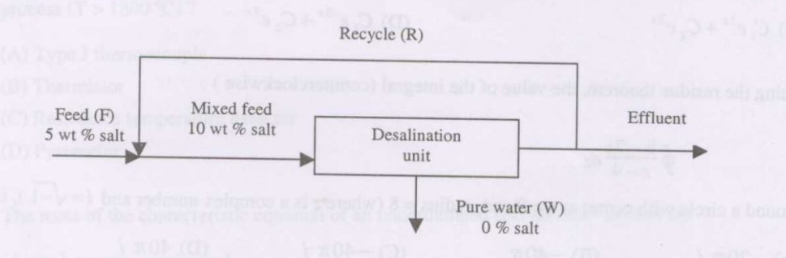
\includegraphics[width = 0.7\columnwidth]{q28.png}
			\caption{}
			\label{fig:Q24}
		\end{figure}
		
		If the overall recovery of pure water \brak{\text{through stream W}} is 0.75 kg/kg feed, then the recycle ratio \brak{R/F} is 
		\begin{enumerate}
			\begin{multicols}{4}
				\item 0.25
				\item 0.5
				\item 0.75
				\item 1.0
			\end{multicols}
		\end{enumerate}
		
		\hfill \brak{\text{GATE CH 2009}}
		
		\item For a binary mixture at constant temperature and pressure, which ONE of the following relations between activity coefficient $\gamma$ and mole fraction $\chi$ is thermodynamically consistent ? 
		\begin{enumerate}
			\item ln $\gamma_1$ = -1+2$\chi_{1}$ - $\chi_{1}^2$, ln $\gamma_{2}$ = $\frac{1}{2}$ $\chi_{1}^2$
			\item ln $\gamma_{1}$ = -1+$\chi_{1}$ - $\chi_{1}^2$, ln $\gamma_{2}$ = $\chi_{1}^2$
			\item ln $\gamma_{1}$ = -1+$\chi_{1}$ - $\chi_{1}^2$, ln $\gamma_{2}$ = $-\frac{1}{2}$ $\chi_{1}^2$
			\item ln $\gamma_{1}$ = -1+$\chi_{1}$ - $\chi_{1}^2$, ln $\gamma_{2}$ = -$\chi_{1}^2$
		\end{enumerate}
		
		\hfill \brak{\text{GATE CH 2009}}
		
		\item Two identical reservoirs, open at the top, are drained through pipes attached to the bottom of the tanks as shown below. The two drain pipes are of the same length, but of different diameters $D_1>D_2$
		
		\begin{figure}[H]
			\centering
			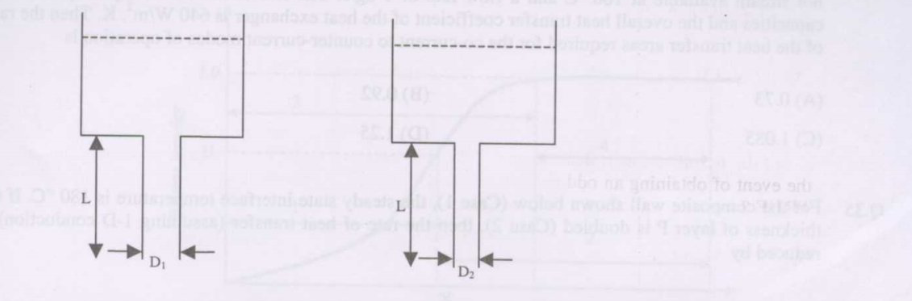
\includegraphics[width = 0.7\columnwidth]{q30.png}
			\caption{}
			\label{fig:Q30}
		\end{figure}
		
		Assuming the flow to be steady and laminar in both drain pipes, if the volumetric flow rate in the larger pipe is 16 times of that in the smaller pipe, the ratio $D_1/ D_2$ is 
		\begin{enumerate}
			\begin{multicols}{4}
				\item 2
				\item 4
				\item 8
				\item 16
			\end{multicols}
		\end{enumerate}
		
		\hfill \brak{\text{GATE CH 2009}}
		
		
		\item For an incompressible flow, the x- and y-components of the velocity vector are $v_{y} = 3\brak{y + z} v_{x} = 2\brak{x + y}$ where x, y, z are in metres and velocities are in m/s. Then the z-component of the velocity vector \brak{v_{z}} of the flow for the boundary condition $v_{z}$ = 0 at z = 0 is 
		\begin{enumerate}
			\begin{multicols}{4}
				\item  5z
				\item  -5z
				\item 2x+3z
				\item -2x-3z
			\end{multicols}
		\end{enumerate}
		
		\hfill \brak{\text{GATE CH 2009}}
		
		\item The terminal settling velocity mm diameter glass sphere \brak{\text{density: $2500$kg / }m^3} in a viscous Newtonian liquid \brak{\text{density: $1500$kg / }m^3 } is 100 s /mu m/s .If the particle Reynolds small and the value of acceleration due to gravity is 9.81m /$s^2$ the viscosity of the liquid \brak{\text{in Pa.s}} is 
		\begin{enumerate}
			\begin{multicols}{4}
				\item 100
				\item 196.2
				\item 245.3
				\item 490.5
			\end{multicols}
		\end{enumerate}
		
		\hfill \brak{\text{GATE CH 2009}}
		
		\item A well-insulated hemispherical furnace \brak{radius= 1m } is shown below: \\
		\begin{figure}[H]
			\centering
			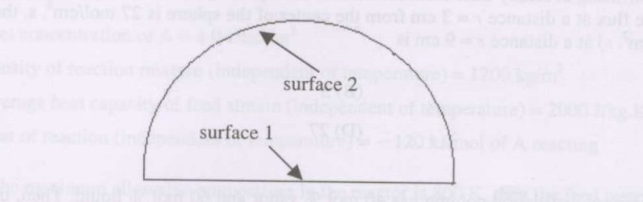
\includegraphics[width = 0.7\columnwidth]{q33.png}
			\caption{}
			\label{fig:Q33}
		\end{figure}
		
		The self-view factor of radiation for the curved surface 2 is 
		\begin{enumerate}
			\begin{multicols}{4}
				\item 1/4
				\item 1/2
				\item 2/3
				\item 3/4
			\end{multicols}
		\end{enumerate}
		
		\hfill \brak{\text{GATE CH 2009}}
		
		\item A double-pipe heat exchanger is to be designed to heat 4 kg/s of a cold feed from 20 to $40\degree C$ using a hot stream available at $160\degree C$ and a flow rate of 1 kg/s. The two streams have equal specific heat capacities and the overall heat transfer coefficient of the heat exchanger is 640W /$m^2$ K. Then the ratio of the heat transfer areas required for the co-current to counter-current modes of operation 
		\begin{enumerate}
			\begin{multicols}{2}
				\item 0.92
				\item 0.73
				\item 1.085
				\item 1.25
			\end{multicols}
		\end{enumerate}
		
		\hfill \brak{\text{GATE CH 2009}}
		
		\item For the composite wall shown below \brak{Case 1}, the steady state interface temperature is $180\degree C$ If the thickness of layer P is doubled \brak{Case 2}, then the rate of heat transfer \brak{\text{assuming 1-D conduction}} is reduced by \\
		\begin{figure}[H]
			\centering
			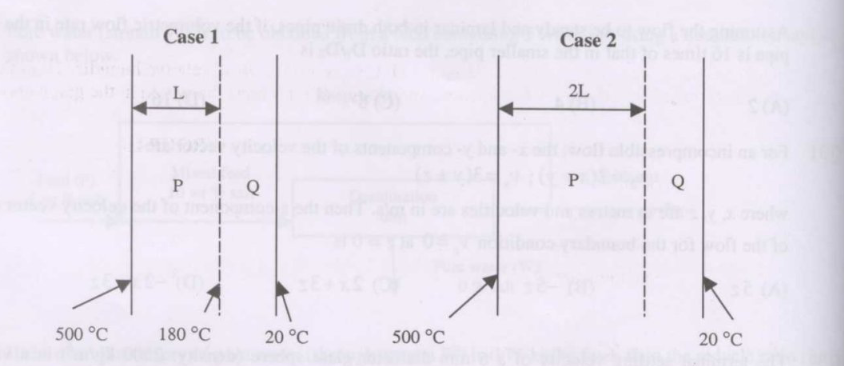
\includegraphics[width = 0.7\columnwidth]{q35.png}
			\caption{}
			\label{fig:Q35}
		\end{figure}
		
		\begin{enumerate}
			\begin{multicols}{2}
				\item 20\%
				\item 40\%
				\item 50\%
				\item 70\%
			\end{multicols}
		\end{enumerate}
		
		\hfill \brak{\text{GATE CH 2009}}
		
		\item Species A is diffusing at steady state from the surface of a sphere \brak{\text{radius }= 1cm } into a stagnant fluid. If the diffusive flux at a distance r = 3 cm from the center of the 27mol / $cm^2$ s, the diffusive flux \brak{\text{in mol/ }cm^2.s} at a distance r = 9 cm is 
		\begin{enumerate}
			\begin{multicols}{2}
				\item 1
				\item 3
				\item 9
				\item 27
			\end{multicols}
		\end{enumerate}
		
		\hfill \brak{\text{GATE CH 2009}}
		
		
		
		\item The feed to a binary distillation column has 40 mol \% vapor and 60 mol \% liquid. Then, the slope of the q-line in the McCabe-Thiele plot is 
		\begin{enumerate}
			\begin{multicols}{4}
				\item -1.5
				\item -0.6
				\item 0.6
				\item 1.5
			\end{multicols}
		\end{enumerate}
		
		\hfill \brak{\text{GATE CH 2009}}
		
		\item The equilibrium moisture curve for a solid is shown below:
		
		\begin{figure}[H]
			\centering
			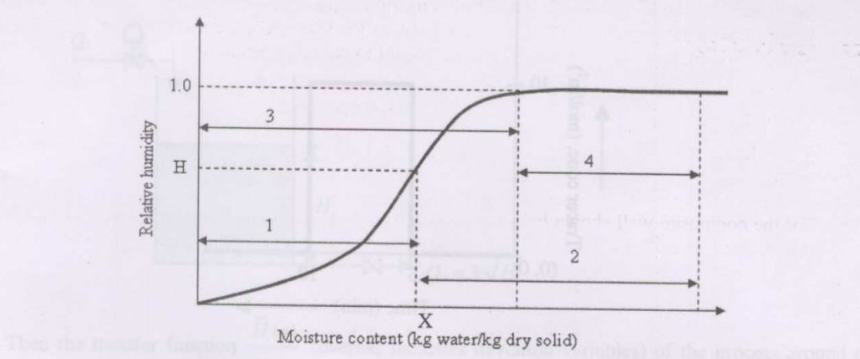
\includegraphics[width = 0.7\columnwidth]{q38.png}
			\caption{}
			\label{fig:Q38}
		\end{figure}
		
		
		The total moisture content of the solid is X and it is exposed to air of relative humidity H. In the table below. Group I lists the types of moisture, and Group II represents the region in the graph above. 
		\begin{center}
			\begin{tabular}{ c c c }
				& \textbf{GROUP I} &\textbf{GROUP II} \\
				P. & Equilibrium moisture & 1 \\
				Q. & Bound moisture & 2 \\ 
				R. & Unbound moisture & 3 \\
				S. & Free moisture & 4 
			\end{tabular}
		\end{center}
		\begin{enumerate}
			\begin{multicols}{2}
				\item P-1, Q-2, R-3, S-4
				\item P-1, Q-3, R-4, S-2
				\item P-1, Q-4, R-2, S-3
				\item P-1, Q-2, R-4, S-3
			\end{multicols}
		\end{enumerate} 
		
		\hfill \brak{\text{GATE CH 2009}}
		
		
		\item The liquid-phase reaction A $\rightarrow$B is conducted in an adiabatic plug flow reactor.
		
		Data:
		\begin{enumerate}
			\item Inlet concentration of A = $4.0 kmol/m^3$
			\item Density of reaction mixture \brak{\text{independent of temperature}} = $1200 kg/m$ Average heat capacity of feed stream \brak{independent of temperature} = 2000 J/kg.K
			\item Heat of reaction \brak{\text{independent of temperature}}120 kJ/mol of A reacting
			\item If the maximum allowable temperature in the reactor is 800 K, then the feed temperature \brak{\text{in K}} should not exceed
		\end{enumerate} 
		\begin{enumerate}
			\begin{multicols}{2}
				\item 400
				\item 500
				\item 600
				\item 700
			\end{multicols}
		\end{enumerate} 
		
		\hfill \brak{\text{GATE CH 2009}}
		
		\item An isothermal pulse test is conducted on a reactor and the variation of the outlet tracer concentration with time is shown below:
		\begin{figure}[H]
			\centering
			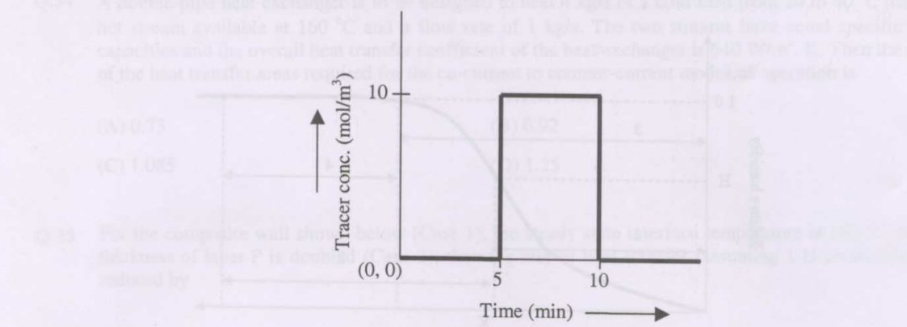
\includegraphics[width = 0.7\columnwidth]{q40.png}
			\caption{}
			\label{fig:Q40}
		\end{figure}
		
		
		
		The mean residence time of the fluid in the reactor \brak{\text{in minutes}} is 
		\begin{enumerate}
			\begin{multicols}{2}
				\item 5.0
				\item 7.5
				\item 10.0
				\item 15.0
			\end{multicols}
		\end{enumerate} 
		
		\hfill \brak{\text{GATE CH 2009}}
		
		
		\item The inverse Laplace transform of is  $\frac{1}{2s^2 + 3s + 1}$ 
		\begin{enumerate}
			\begin{multicols}{2}
				\item $e^\frac{-t}{2}$ - $e^-t$ 
				\item $2e^\frac{-t}{2}$ - $e^-t$ 
				\item $e^\frac{-t}{2}$ - $2e^-t$
				\item $e^\frac{-t}{2}$ - $e^-t$ 
			\end{multicols}
		\end{enumerate} 
		
		\hfill \brak{\text{GATE CH 2009}}
		
		
		\item The characteristic  of a closed loop system using a proportional controller with gain $K_{c}$ is
		\begin{equation*}
			12s ^ 3 + 19s ^ 2 + 8s + 1 + K_{c} = 0
		\end{equation*}
		
		At the onset of instability, the value of $K_{c}$ is 
		\begin{enumerate}
			\begin{multicols}{4}
				\item 35/3
				\item 10
				\item 25/3
				\item 20/3
			\end{multicols}
		\end{enumerate} 
		
		\hfill \brak{\text{GATE CH 2009}}
		
		\item The block diagram for a control system is shown below:
		\begin{figure}[H]
			\centering
			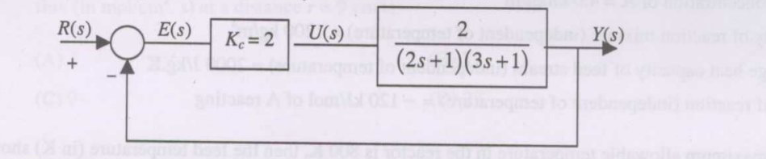
\includegraphics[width = 0.7\columnwidth]{q43.png}
			\caption{}
			\label{fig:Q43}
		\end{figure}
		
		For a unit step change in the set point, R\brak{s} the steady state offset in the output Y\brak{s} is 
		\begin{enumerate}
			\begin{multicols}{4}
				\item 0.2
				\item 0.3
				\item 0.4
				\item 0.5
			\end{multicols}
		\end{enumerate} 
		
		\item For a tank of cross-sectional area 100$cm^2$ and inlet flow rate \brak{ Q_{i} \text{ in } cm^3/s } , the outlet flow rate \brak{Q_{o} \text{ in } cm^3/s} is related to the liquid height \brak{\text{H in cm as}} $Q_{o} = 3\sqrt{\brak{H}}$ \brak{\text{see figure below}}.
		
		\begin{figure}[H]
			\centering
			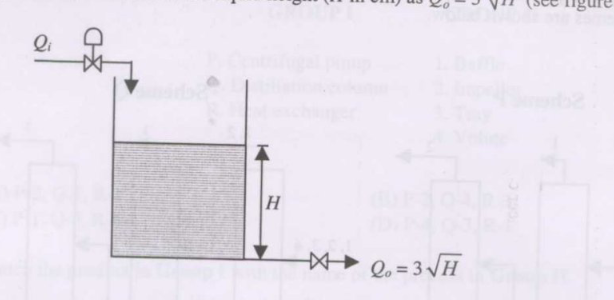
\includegraphics[width = 0.7\columnwidth]{q44.png}
			\caption{}
			\label{fig:Q44}
		\end{figure}
		
		Then the transfer function $\frac{H\brak{s}}{Q\brak{S}}$ of the process around the steady-state point, $Q_{Lx}$ =18$cm^3$/s and $H_{x}$ = 36cm is 
		\begin{enumerate}
			\begin{multicols}{2}
				\item $\frac{1}{100s+1}$
				\item $\frac{2}{200s+1}$
				\item $\frac{3}{300s+1}$
				\item $\frac{4}{400s+1}$
			\end{multicols}
		\end{enumerate} 
		
		\hfill \brak{\text{GATE CH 2009}}
		
		
		\item A column costs Rs. 5.0 lakhs and has a useful life of 10 years. Using the double declining balance depreciation method, the book value of the unit at the end of five years \brak{\text{in lakhs of Rs.}} is 
		\begin{enumerate}
			\begin{multicols}{2}
				\item 1.21
				\item 1.31
				\item 1.64
				\item 2.05
			\end{multicols}
		\end{enumerate} 
		
		\hfill \brak{\text{GATE CH 2009}}
		
		\item An equi-molar mixture of four hydrocarbons \brak{1, 2, 3, 4} is to be separated into high purity individual components using a sequence of simple distillation columns \brak{\text{one overhead and one bottom stream}}. Four possible schemes are shown below.
		\begin{figure}[H]
			\centering
			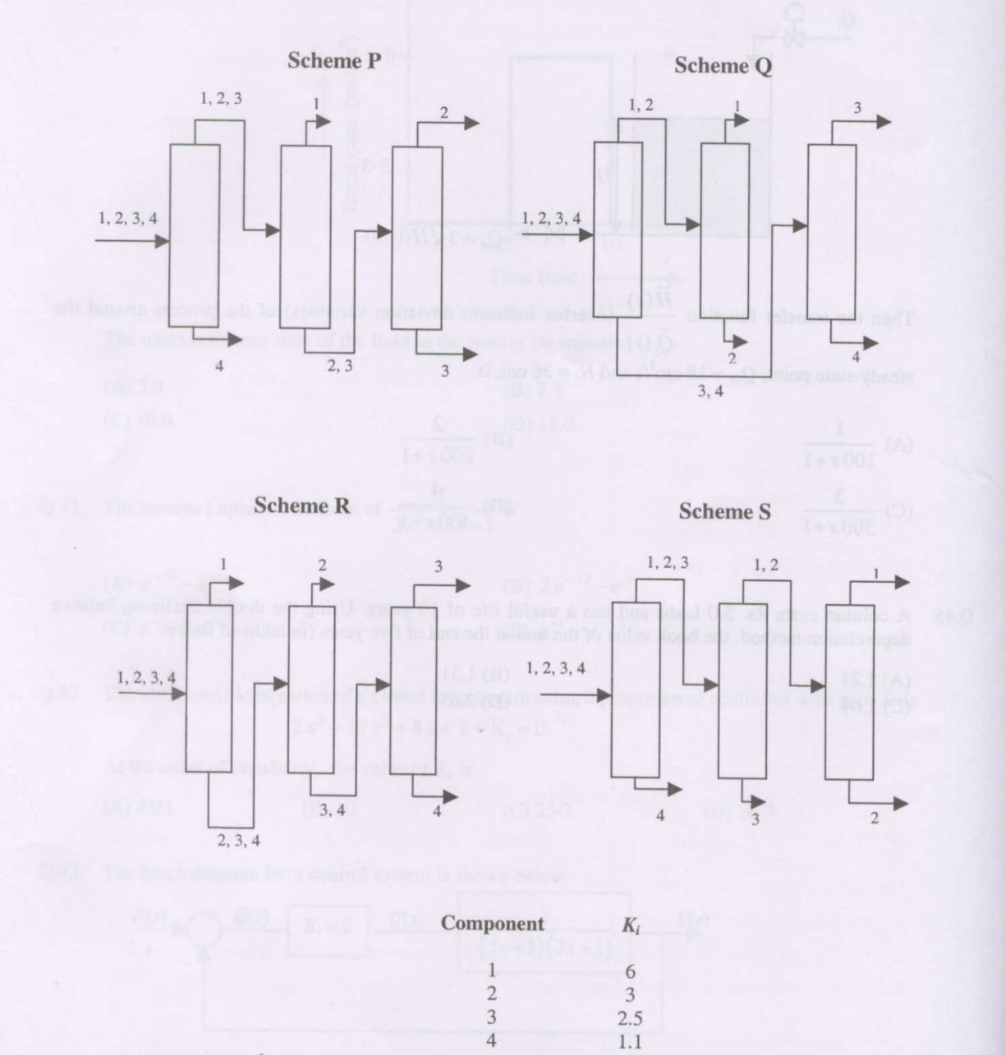
\includegraphics[width = 0.7\columnwidth]{q46.png}
			\caption{}
			\label{fig:Q46}
		\end{figure}
		\begin{center}
			\begin{tabular}{ c c }
				\textbf{Component} &\textbf{$K_{i}$} \\
				1 & 6 \\
				2 & 3 \\
				3 & 2.5 \\
				4 & 1.1
			\end{tabular}
		\end{center} 
		
		\begin{enumerate}
			\begin{multicols}{4}
				\item P
				\item Q
				\item R
				\item S
			\end{multicols}
		\end{enumerate} 
		
		\hfill \brak{\text{GATE CH 2009}}
		
		
		\item Match the equipment in Group I to the internals in Group II 
		\begin{center}
			\begin{tabular}{ c c c c }
				& \textbf{GROUP I} &  &\textbf{GROUP II} \\
				P. & Centrifugal Pump & 1. & Baffle \\
				Q. & Distillation column & 2. & Impeller \\
				R. & Heat exchanger & 3. & Tray \\
				& & 4. & Volute
			\end{tabular}
		\end{center} 
		
		\begin{enumerate}
			\begin{multicols}{2}
				\item P-2, Q-1, R-4
				\item P-2, Q-4, R-3
				\item P-1, Q-3, R-4
				\item P-4, Q-3, R-1
			\end{multicols}
		\end{enumerate} 
		
		\hfill \brak{\text{GATE CH 2009}}
		
		
		
		\item Match the product in Group I with the name of the process in Group II.
		\begin{center}
			\begin{tabular}{ c c c c }
				& \textbf{GROUP I} &  &\textbf{GROUP II} \\
				P. & Sodium carbonate & 1. & Haber \\
				Q. & Ammonia & 2. & Solvay \\
				R. & Sulphuric acid & 3. & Fischer-Tropsch \\
				& & 4. & Contact
			\end{tabular}
		\end{center} 
		\begin{enumerate}
			\begin{multicols}{2}
				\item P-2, Q-1, R-4
				\item P-4, Q-1, R-2
				\item P-3, Q-4, R-2
				\item P-2, Q-1, R-3
			\end{multicols}
		\end{enumerate} 
		
		\hfill \brak{\text{GATE CH 2009}}
		
		\item Match the product in Group I to the raw material in Group II.
		\begin{center}
			\begin{tabular}{ c c c c }
				& \textbf{GROUP I} &  &\textbf{GROUP II} \\
				P. & Ethylene & 1. & Natural gas\\
				Q. & Methanol & 2. & Synthesis gas \\
				R. & Pthalic anhydride & 3. & Naphtha \\
				& & 4. & Naphtalene
			\end{tabular}
		\end{center} 
		\begin{enumerate}
			\begin{multicols}{2}
				\item P-1, Q-2, R-3
				\item P-2, Q-1, R-4
				\item P-3, Q-1, R-4
				\item P-3, Q-2, R-4
			\end{multicols}
		\end{enumerate} 
		
		\hfill \brak{\text{GATE CH 2009}}
		
		\item Match the unit process in Group I with the industry in Group II.
		\begin{center}
			\begin{tabular}{ c c c c }
				& \textbf{GROUP I} &  &\textbf{GROUP II} \\
				P. & Steam cracking & 1. & Petroleum refining \\
				Q. & Hydrocracking & 2. & Petrochemicals \\
				R. & Condensation & 3. & Polymers \\
				& & 4. & Soaps and detergents
			\end{tabular}
		\end{center} 
		\begin{enumerate}
			\begin{multicols}{2}
				\item P-1, Q-2, R-3
				\item P-2, Q-3, R-3
				\item P-1, Q-2, R-4
				\item P-2, Q-1, R-3
			\end{multicols}
		\end{enumerate} 
		
		\hfill \brak{\text{GATE CH 2009}}
		
		
		\newpage 
		
		\textbf{Common Data for Questions 51 and 52}
		An ideal gas with molar heat capacity $C_{p}$ = $5/2\times R$ \brak{where R = 8.314 J/mol K} is compressed adiabatically from 1 bar and 300 K to pressure $P_{2}$ in a closed system. The final temperature after compression is 600 K and the mechanical efficiency of compression is 50\%.
		\item The work required for compression \brak{\text{in kJ / mol} } is 
		\begin{enumerate}
			\begin{multicols}{4}
				\item 3.74
				\item 6.24
				\item 7.48
				\item 12.48
			\end{multicols}
		\end{enumerate} 
		
		\hfill \brak{\text{GATE CH 2009}}
		
		
		\item The final pressure $P_{2}$ \brak{\text{in bar}} is 
		\begin{enumerate}
			\begin{multicols}{4}
				\item $2^\frac{3}{4}$
				\item $2^\frac{5}{4}$
				\item $2^\frac{3}{2}$
				\item $2^\frac{5}{2}$
			\end{multicols}
		\end{enumerate}
		
		\hfill \brak{\text{GATE CH 2009}}
		
		\textbf{Common Data for questions 53 and 54}
		
		A slab of thickness L with one side \brak{x = 0} insulated and the other side \brak{x = L} maintained at a constant temperature $T_{0}$ is shown below. \\
		\begin{figure}[H]
			\centering
			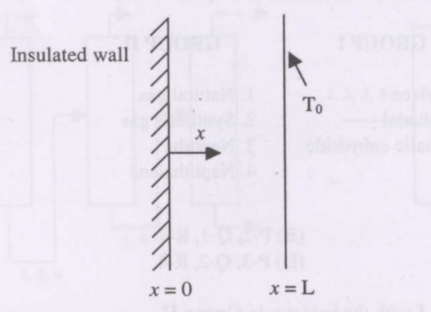
\includegraphics[width = 0.7\columnwidth]{q53.png}
			\caption{}
			\label{fig:Q53}
		\end{figure}
		
		A uniformly distributed internal heat source produces heat in the slab at the rate of SW / $m^3$ Assume the heat conduction to be steady and 1-D along the x-direction.
		
		\item The maximum temperature in the slab occurs at x equal to 
		\begin{enumerate}
			\begin{multicols}{4}
				\item 0
				\item L/4
				\item L/2
				\item L
			\end{multicols}
		\end{enumerate}
		
		\hfill \brak{\text{GATE CH 2009}}
		
		\item The heat flux at x = L is 
		\begin{enumerate}
			\begin{multicols}{4}
				\item 0
				\item S L/4
				\item S L/2
				\item S L
			\end{multicols}
		\end{enumerate}
		
		\hfill \brak{\text{GATE CH 2009}}
		
		
		\textbf{Common Data for Questions 55 and 56}
		A flash distillation drum \brak{\text{see figure below}} is used to separate a methanol-water mixture. The mole fraction of methanol in the feed is 0.5, and the feed flow rate is 1000 kmol/hr. The feed is preheated in a heater with heat duty Q and is subsequently flashed in the drum. The flash drum can be assumed to be an equilibrium stage, operating adiabatically. The equilibrium relation between the mole fractions of methanol in the vapor and liquid phases is y = 4 x. The ratio of distillate to feed flow rate is 0.5.
		\begin{figure}[H]
			\centering
			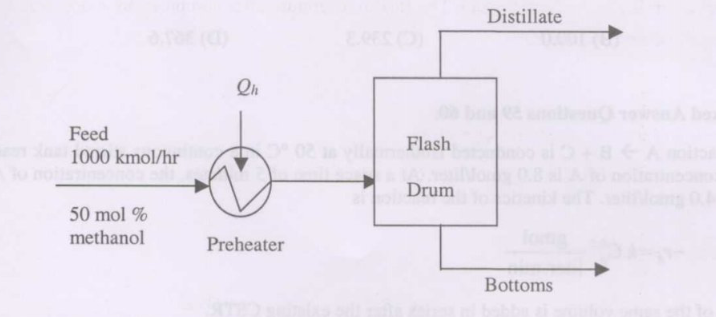
\includegraphics[width = 0.5\columnwidth]{q55.png}
			\caption{}
			\label{fig:Q55}
		\end{figure}
		
		\item The mole fraction of methanol in the distillate is
		\begin{enumerate}
			\begin{multicols}{4}
				\item 0.2
				\item 0.7
				\item 0.8
				\item 0.9
			\end{multicols}
		\end{enumerate}
		
		\hfill \brak{\text{GATE CH 2009}}
		
		\item If the enthalpy of the distillate with reference to the feed is 3000 kJ/kmol, and the enthalpy of the bottoms with reference to the feed is -1000 kJ/kmol, the heat duty of the preheater \brak{\text{Q in kJ / hr }} is 
		\begin{enumerate}
			\begin{multicols}{4}
				\item $-2\times10^6$
				\item $-1\times10^6$
				\item $1\times10^6$
				\item $2\times10^6$
			\end{multicols}
		\end{enumerate}
		
		\hfill \brak{\text{GATE CH 2009}}
		
		\textbf{Statement for Linked Answer Questions 57 and 58}
		
		A free jet of water is emerging from a nozzle \brak{\text{diameter 75 mm}} attached to a pipe \brak{\text{diameter 225 mm}} as shown below.
		
		\begin{figure}[H]
			\centering
			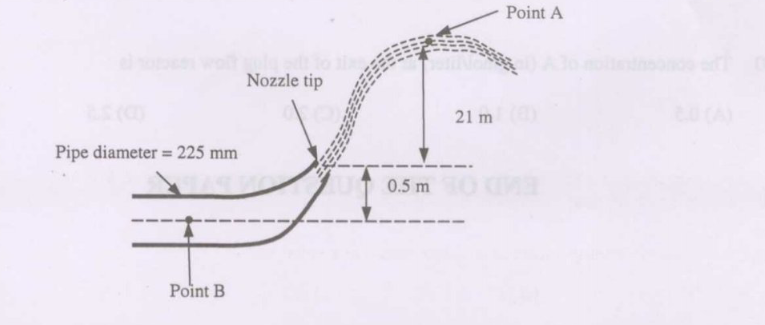
\includegraphics[width = 0.7\columnwidth]{q57.png}
			\caption{}
			\label{fig:Q57}
		\end{figure}
		
		The velocity of water at point A is 18 m/s. Neglect friction in the pipe and nozzle. Use g = 9.81 $m/s^2$ and density of water = $1000 kg/m^3$.
		
		
		\item The velocity of water at the tip of the nozzle \brak{\text{in m / s}} is
		\begin{enumerate}
			\begin{multicols}{4}
				\item 13.4
				\item 18.0
				\item 23.2
				\item 27.1
			\end{multicols}
		\end{enumerate} 
		
		\hfill \brak{\text{GATE CH 2009}}
		
		\item The gauge pressure \brak{\text{in kPa}} at point B is  
		\begin{enumerate}
			\begin{multicols}{4}
				\item 80.0
				\item 100.0
				\item 239.3
				\item 367.6
			\end{multicols}
		\end{enumerate}
		\hfill \brak{\text{GATE CH 2009}}
		
		
		\textbf{Statement for Linked Answer Questions 59 and 60}
		\\ The liquid-phase reaction A $\rightarrow $B + C is conducted isothermally at $50\degree C$ in a continuous stirred tank reactor \brak{CSTR}. The inlet concentration of A is 8.0 gmol/liter. At a space time of 5 minutes, the concentration of A at the exit of CSTR is 4.0 gmol/liter. The kinetics of the reaction is
		
		$-r_{A}$ = k$^{0.5}C_A \frac{gmol}{liter.min}$
		
		A plug flow reactor of the same volume is added in series after the existing CSTR.
		\item The rate constant \brak{k} for this reaction at $50\degree C$ is 
		\begin{enumerate}
			\begin{multicols}{2}
				\item $0.2\brak{\frac{gmol}{liter}}^{0.5}{} min^{-1}$
				\item $0.2\brak{\frac{gmol}{liter}}^{0.5}{} min^{-1}$
				\item $0.4\brak{\frac{gmol}{liter}}^{0.5}{}min^{-1}$
				\item $0.4\brak{\frac{gmol}{liter}}^{0.5}{}min^{-1}$
			\end{multicols}
		\end{enumerate}
		
		\hfill \brak{\text{GATE CH 2009}}
		
		\item The concentration of A \brak{\text{in gmol/liter}} at the exit of the plug flow reactor is 
		\begin{enumerate}
			\begin{multicols}{4}
				\item $0.5$
				\item $1.0$
				\item $2.0$
				\item $2.5$
			\end{multicols}
		\end{enumerate}
		
		\hfill \brak{\text{GATE CH 2009}}
		
	\end{enumerate}
\end{document}
